\chapter{Minimization of a Functional}

A classical problem in minimization is the brachistrochrone, so the fastest ultimate curve (meaning determining the fastest trajectory to move from a point $A$ to a point $B$ considering that the only action is the one of the gravity).

\begin{SCfigure}[3][bht]
	\centering 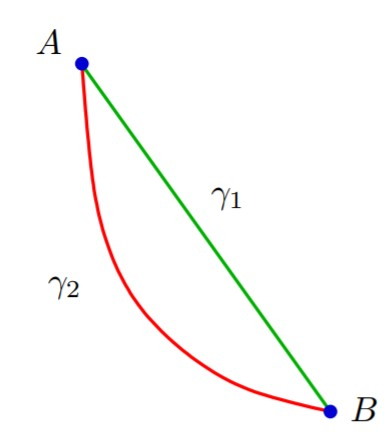
\includegraphics[width=2.5cm]{brachi}
	\caption{example of two trajectories $\gamma_1,\gamma_2$ that an object can follow for moving from point $A$ to $B$.}
\end{SCfigure}

Mathematically the problem is determining the curve $\mathcal C: [a,b] \rightarrow \mathds R$ such that $\mathcal C(a) = y_a$ and $\mathcal C(b) = y_b$ that minimize the function $T(\mathcal C)$ representing the time to travel and so
\[ \textrm{minimize } T(\mathcal C) \qquad \textrm{for all possible curves } \mathcal C \]

We can see that a \textbf{function} takes a number as input and returns a number, like $f(x) = x e^x$. A \de{functional} is instead something that takes as input a function and returns a number and an example is
\[ \mathcal F (x) = \int_a^b x(t)\, dt  \]
where $x$ is a function. Considering for example $x(t) = t^2$ the previous functional  becomes
\[ \fun F(x) = \int_a^b t^2\, dt = \left. \frac{t^3}{3}\right|_a^b= \frac{b^3-a^3}{3}\]

Another example of functional can be $\fun G(z) = z'(0) \int_0^1 z^2(t)\, dt$ and this expression can be evaluated for every generic function $z(t)$.	\vspace{3mm}

The question of this problem is how to define a \textit{minimum} for a functional; in order to do so we have to firstly understand how to minimize a simple function and in particular given a function $f: A\subseteq \R \rightarrow \R$ has a minimum in the point $x^*$ if
\[  f(x^*) \leq f(x) \qquad \forall x \in A \]
Similarly given a function $\fun F(x)$ a \textit{point} $x^*$ (that in reality is a function) is a minimum if 
\[ \fun F(x^*) \leq \fun F(x) \qquad \forall x \in ? \]
In this case we have to specify the \textit{class} (functional space) of functions we are considering, as example $x$ can be a function that's continuous in the domain $[a,b]$ and so we can define
\[ x\in C([a,b]) = \big\{ g:[a,b]\rightarrow R \ | \ g \textrm{ is continuous} \big\} \]
In general changing the \textit{domain} of the functional $\fun F$ may change the problem.
\begin{example}{: domain change}
	Considering the function $f(x) = x^2+2$, it's roots can be computed if we allow complex solutions $z\in \mathds C$ (and in fact $z = \pm i \sqrt 2$), while if the domain of the solution is the real set $z\in \R$ no solutions exists. \vspace{3mm}
	
	Considering now the functional $\fun F$ defined as
	\[ \fun F(x) = \int_{-1}^1 \big(x(t) - |t|\big)^2\, dt \]
	The $|t|$ introduce a cuspid in $t=0$ that cannot be derived. If we minimize the functional in the continuous interval $x\in C([-1,1])$, the solution is the function $x^*(t) = |t|$, in fact
	\[ \fun F(x^*) = \int_{-1}^1 \big(|t|-|t|\big)^2 \, dt = \int_{-1}^1 0\, dt = 0 \]
	Choosing any other continuous function will result in a functional with a positive value.
	
	Considering now to minimize the function in the domain of functions with continuous derivatives, and so $x\in C^1([-1,1])$. In this case $|t|\notin C^1([-1,1])$ (due to the cuspid). An approximation of the function $|t|$ that is continuous with also continuous first derivative is the function
	\[ x_\varepsilon(t) = \begin{cases}
		t \qquad & t \geq \varepsilon \\
		\frac 1 2 \left(\frac{t^2}\varepsilon + \varepsilon\right) \qquad & -\varepsilon < t< \varepsilon \\
		-t & t \leq- \varepsilon
	\end{cases} \]
	By pushing the limit $\varepsilon\rightarrow 0$ we can have the function that minimize the functional $\fun F$ in the domain $C^1([-1,1])$. In fact we can see that the functional of $x_\varepsilon$ becomes
	\[ \fun F(x_\varepsilon) = \int_{-\varepsilon}^\varepsilon \left( \frac{t^2}{2\varepsilon} + \frac \varepsilon 2 - |t| \right)^2\, dt = \frac{\varepsilon^3}{10} \]
	
\end{example}

\section{Analogies with linear algebra}
To solve the problem of minimizing a functional we can see some relations with the linear algebra. The domain of the functional can be in fact see as a \de{functional space} $\mathds V$ analogous to the vectorial one which the vectors are represented by the functions and the scalars are represented by real values. With this definition example of functional spaces might be
\[ \mathds V_1 = \big\{ f : [0,1] \rightarrow \R \textrm{ continuous}\big\} \]
\[ \mathds V_2 = \big\{ f: [a,b]\rightarrow \R \textrm{ such that } f\in C^k([a,b]) \big\} \qquad \textrm{with } a,b \in \R, \ k\in \mathds N \]
Given in fact two function $f,g \in \mathds V$ that are member of the same functional space, we can see that each linear combination of the functions determine a function that's still in the vectorial space:
\[ \alpha f(x) + \beta f(x) \in \mathds V \qquad \forall \alpha,\beta \in \R, \ f(x),g(x) \in \mathds V \]
As example let's consider the two continuous function $f(x) = x^2$ and $g(x) = \sin x$, then we can clearly see that the function $2f(x) + \frac 13 g(x) = 2x^2 +\frac 13\sin x$ is still continuous. This in general means that the functional space is \textit{closed} respect to the operations of function summation and multiplication by a scalar.

\paragraph{Scalar product} In linear algebra given two vector $\vett v_1, \vett v_2$ it exists the bilinear operator scalar product $\langle \vett v_1,\vett v_2 \rangle = \vett v_1 \cdot \vett v_2$  that satisfy the following rules:
\[ \langle \alpha \vett v + \beta \vett w, \vett z\rangle = \langle \vett z , \alpha \vett v + \beta \vett w\rangle = \alpha \langle \vett v,\vett z\rangle + \beta \langle \vett w,\vett z\rangle \qquad \forall \alpha,\beta \in \R, \ \vett v,\vett w,\vett z \in \mathds V \]	
\[ \langle \vett v,\vett v\rangle \geq 0 \qquad \textrm{ and } \qquad \langle \vett v,\vett v \rangle = 0 \quad \Leftrightarrow \quad \vett v = \vett 0 \]

Also in the functional space $\mathds V$ can exists definitions of product scalar such the one here presented:
\begin{equation} \label{eq:func:pscalexample}
	\langle f,g\rangle = \int_0^1 f(x)g(x)\, dx
\end{equation}
\begin{note}
	This is not the lonely function that can serve as product scalar of function and in this case the relation holds for the functional space $\mathds V = \{ f:[0,1] \rightarrow \R \textrm{ integrable} \}$.
\end{note}
In this case we can prove that this definitions meets the requirements stated for the scalar product considering the linear properties of the integrals as follows:
\begin{align*}
	\langle \alpha f(x) + \beta g(x),h(x) \rangle & = \int_0^1 \Big(\alpha f(x) + \beta g(x)\Big)h(x) \, dx \\ 
	& = \alpha \int_0^1 f(x)h(g) \, dx + \beta \int_0^2 g(x)h(x) \, dx \\
	& = \alpha \langle f(x),h(x) \rangle + \beta \langle g(x),h(x) \rangle
\end{align*}
and also
\[ \langle f(x),f(x) \rangle = \int_0^1 f(x) f(x) \, dx = \int_0^1 f^2(x)  \geq 0  \]
and in particular we can see that the scalar product $\langle f(x),f(x)\rangle$ will give as result 0 if and only if the function $f$ is identically null, so such that $f(x) = 0$ for all $x$ in it's domain (in this case $[0,1]$).

\paragraph{Norm} In linear algebra it's also defined the norm of a vector as
\[ \|\vett v\| := \sqrt{\vett v \cdot \vett v} \]
and this expression is used to compute, from a vector, a single positive value  (and in particular $\|\vett v\| = 0$ if and only if $\vett v = \vett 0$). This definition also holds for the functional space and considering the scalar product defined (as example) in equation \ref{eq:func:pscalexample} we can see that one definition of norm for function can be the one
\[ \|f(x)\| = \sqrt{\langle f(x),f(x)\rangle} = \sqrt{\int_0^1f^2(x) \, dx} \]
In this case we can clearly see that the norm $\|f(x)\| \geq 0$ is always positive defined (and is zero only in the case on which the function $f$ is identically null).


\begin{example}{: space of function}
	A space of functions can ve the one $f:[a,b]\rightarrow \R$ such that $f$ is continuous, or for example $f:[a,b]\rightarrow \R$ where $f\in C^k([a,b])$ (for $k\in \mathds N$). The same can be said for piecewise continuous functions.
	
	Less trivially is a space of function the set of $f:[a,b]\rightarrow \R$ that are module integrable, and so all the function $f$ such that
	\[\int_a^b |f(x)|\, dx < \infty\]
	
\end{example}

In general we define as $L^p([a,b])$ the space of $p$-integrable functions, so such that
\[ f\in L^p([a,b])  \qquad \Leftrightarrow \qquad \int_a^b |f(x)|^p\, dx < \infty\]


\section{First variation}
	
	Given a functional $\mathcal J: \mathds V\rightarrow \R$ defined in the function space $\mathds V$, in order to determine the first necessary condition for minimum of the function we have to define the concept of \textbf{derivative} for functionals that is called (\de{first}) \de{variation} (or \textbf{directional derivative}).

	To determine the first variation of the functional $\mathcal J$ respect to the function $x\in \mathds V$ we have to define to compute the functional for the function $x + \alpha \eta$, where $\eta \in \mathds V$ (and can be regarded as the \textit{\textbf{direction} of the derivative}) and $\alpha \in \R$. We can now denote the \textbf{first variation} as $\delta \mathcal J\big|_x:\mathds V\rightarrow \R$ as the function that satisfy the following relation:
	\begin{equation}
		\mathcal J\big(x + \alpha \eta\big) = \mathcal J\big(y\big) + \delta \mathcal J\big|_x(\eta)\alpha +  o(\alpha)
	\end{equation}
	
	By using the definition of the small-$o$ it's possible to express the limit relation that determines the first variation of the function as
	\begin{equation}
		\delta \mathcal J\big|_x (\eta) = \lim_{\alpha\rightarrow 0} \frac{\mathcal J\big(x + \alpha \eta\big) - \mathcal J\big(x\big)}{\alpha}
	\end{equation}
	By so defining the function $g(\alpha) = \mathcal J\big(x+ \alpha \eta \big)$	thein it means that the first variation of the functional $\mathcal J$ respect the function $x$ can be computed as
	\begin{equation} \label{eq:func:dirderivative}
		\delta \mathcal J\big|_x(\eta) = g'(0)
	\end{equation}
	
	
	\begin{example}{: directional derivative of a functional (first variation)}
		Given the functional
		\[ \fun F(x) = \int_0^1 \Big(x^2(t) + 1\Big) \, dt  \ + x(1) \]
		it's first variation respect to a generic direction $d(t)$ can be calculated by firstly determining the associated function $g:\R\rightarrow \R$ defined as
		\begin{align*}
			g(\alpha) &  = \F\big(x(t) + \alpha\, d(t)\big) \\
			& = \int_0^1 \Big( \big(x(t) + \alpha\, d(t)\big)^2 + 1 \Big)\, dt  + x(1) + \alpha\, d(1)
		\end{align*}
	
		As reported in equation \ref{eq:func:dirderivative}, the first variation of the functional $\fun F$ can be regarded as the derivative of $g$ respect to $\alpha$ evaluated for $\alpha = 0$; the first step is so determining
		\[ g'(\alpha ) = \frac{d}{d\alpha}g(\alpha) = \frac d{d\alpha } \int_0^1 \Big( \big(x(t) + \alpha\, d(t)\big)^2 + 1 \Big)\, dt  +  \frac d{d\alpha} \Big(x(1) + \alpha\, d(1)\Big) \]		
		Assuming that $\frac d{d\alpha}\int = \int \frac d{d\alpha}$ (operation that cannot always be performed) then the derivative of $g$ can be regarded as
		\begin{align*}
			g'(\alpha) &= \int_0^1 \frac d{d\alpha} \Big(x(t) + \alpha\, d(t)\Big)^2\, dt + \frac d{d\alpha} \Big(x(1) + \alpha \, d(1)\Big) \\
			& = \int_0^1 2\big(x(t) + \alpha\, d(t)\big) d(t)\, dt + d(1) 
		\end{align*}
	
		Evaluating this expression for $\alpha = 0$ then the first variation of $\fun F$ with direction $d(t)$ becomes
		\[ \delta \fun F\big|_x(d) = g'(0) = \int_0^1 2x(t)d(t)\, dt + d(1) \]
	\end{example}
	
	\subsection{Optimality condition}
		Considering the minimization of a a function $f:A\subseteq \R^n\rightarrow \R$, it has been shown that the first order necessary condition for a point $\vstar x \in A$ to be a minimum point is that it's gradient $\nabla f(\vstar x)$ (the \textit{derivative}) must be null. Similarly in calculus of variation it's proven that the \textbf{first order necessary condition} for the \textbf{optimality} of the solution is that the first variation of the functional $\mathcal J$ must be 
		\begin{equation}
			\delta \mathcal J\big|_x(\eta)= 0
		\end{equation}
		for every \textit{admissible perturbation} $\eta$. \\ In particular we define a \textbf{perturbation} $\eta \in \mathds V$ \textbf{admissible} for the functional $\mathcal J \in A\subseteq \mathds V$ respect to the function $y^*$ if it happens that $y^* + \alpha \eta \in A$ for all value $\alpha$ \textit{sufficiently close to $0$}.


\section{Fundamental lemma of the calculus of variations}
	{\itshape Given a function $f:[a,b]\rightarrow \R$ (piecewise continuous) such that for all $g:[a,b] \rightarrow \R$ continuous (and more in particular $g \in C^\infty([a,b])$ to have a more general definition ) with $g(a) = g(b) = 0$ and $g^{(k)}(a) = g^{(k)}(b) = 0 \ \forall k$, if the integral 
		\begin{equation} \label{eq:func:lemma}
			\int_a^b f(x)\,g(x) \, dx = 0
		\end{equation}
		then $f(x)= 0 $ is identically null. }
	
	\paragraph{Lemma: sign permanence} In order to later proof the fundamental lemma yet described, we have to remark the \textit{sign permanence} that states: {\itshape given a function $f:[a,b]\rightarrow \R$ continuous such that $f(c) >0$, then there exists a $\delta >0$ such that }
	\[ f(x) \geq \frac{f(c)}{2} \qquad \forall x \in [c-\delta,c+\delta] \]
	
	The proof of this lemma can be done defining the parameter $\epsilon = f(c) / 2$; based on the assumption that $f(x)$ is continuous, then
	\[ \exists \delta >0 \qquad \textrm{such that} \qquad |f(x) - f(c)| \leq \varepsilon = \frac{f(c)}{2} \qquad \forall |c-x|\leq \delta \]
	Expanding the module operation the inequality becomes:
	\[ -\frac{f(c)}{2} = - \epsilon \leq f(x)-f(c) \leq \epsilon = \frac{f(c)}{2} \]
	\[ \Rightarrow \qquad \underbrace{-\frac{f(c)}{2} + f(c) \leq f(x)}_{\frac{f(c)}{2} \leq f(x)} \leq f(c) + \frac{f(c)}{2} \]
	and so we prove the lemma of sign permanence.
	
	\paragraph{Proof of the fundamental lemma} The proof of the fundamental lemma of the calculus of variation can be done by contradiction. Let consider the integral $\int_a^b f(x) g(x)\, dx = 0$ for all functions $g(x)$ and such that, given the function $f$, exists a point $c$ such that $f(c) > 0$ (in general the proof can be done for $f(c)\neq 0$). from the sign permanence lemma we can state that exists an interval $[c-\delta,c+\delta]$ such that $f(x) \geq \frac{f(c)}{2 } \geq 0$. Determining the function $g$ as
	\[ g(x) = \begin{cases}
		\dfrac{x-(c-\delta)}{\delta} \qquad & x\in [c-\delta, c] \\
		\dfrac{c-x+\delta}{\delta} & x\in[c,c+\delta] \\
		0 & \textrm{otherwise}
	\end{cases} \]
	Note that this function is continuous but $g\notin C^\infty$ (later will be described a function that presents this feature). With this definition the integral $\int_a^b fg\, dx$ so becomes
	\begin{align*}
		\int_{c-\delta}^{c+\delta} f(x)g(x)\, dx & \geq \frac{f(c)}{2} \int_{c-\delta}^{c+\delta} g(x)\, dx \\
		& \geq \frac{f(c)}{2}\frac \delta 2 > 0
	\end{align*}
	We can clearly see that the integral $\int_a^b fg\, dx$ has a positive real value grater than zero that's (considering that $f$ has at least on point $c$ such that $f(c) >0$) in contraposition with the initial request that the integral should have been zero evaluated. \vspace{3mm}
	
	To create a direction function $g$ that's in the set $C^\infty$ we can use the function $h$(for whose those condition is demonstrated) as in figure \ref{fig:func:ht} defined as:
	\begin{equation} \label{eq:func:ht}
		h(t) = \begin{cases}
			e^{-1/t} \qquad & t > 0 \\ 
			0 & t\leq 0
		\end{cases}
	\end{equation}
	\begin{SCfigure}[2][bt]
		\centering 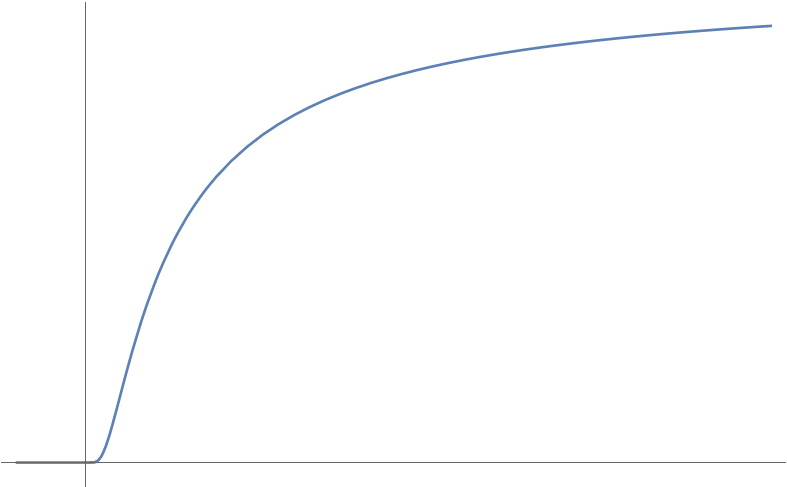
\includegraphics[width=4cm]{cinf-a}
		\caption{representation of $h(t)$ defined in equation \ref{eq:func:ht}}.
		\label{fig:func:ht}
	\end{SCfigure}
	
	A way to create a function that presents a \textit{bell shape} in the range $[0,1]$ is by computing $g(t) := h(t) h(1-t)$ how's graph in the range $[0,1]$ is similar to the one shown in figure \ref{fig:func:hbell}.
	
	\begin{SCfigure}[2][bht]
		\centering 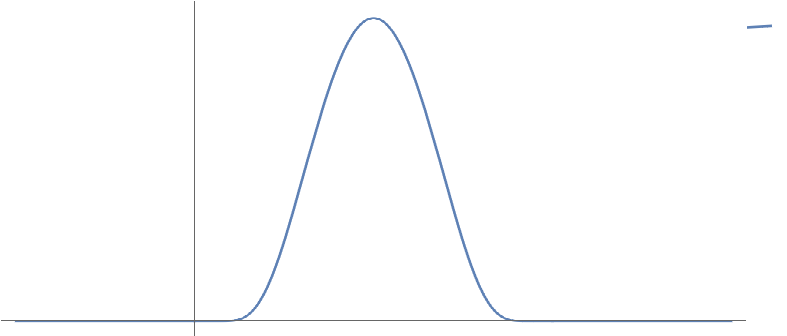
\includegraphics[width=4cm]{cinf-b}
		\caption{representation of the function $g(t):=h(t)h(1-t)$, where $h(t)$ is defined in equation \ref{eq:func:ht}}.
		\label{fig:func:hbell}
	\end{SCfigure}
	
	In particular to demonstrate the fundamental lemma of the calculus of variations we need to rescale the function $g$ in order to have a bell centered in the point $c$ with a \textit{bell width} $\delta$ and so we consider
	\[ g(t) = K \, h\left(\frac{t-c+\delta}{2 \delta}\right) h\left( \frac{\delta + c - t}{2 \delta} \right) \] 
	where the constant $K\in\R$ is such that $g(c)=1$ and $\int_a^bg(x)\, dx$. In this case we can see that $g\in C^\infty$, $g(x) \geq 0 $ for all value $x$ and specifically $g(x) = 0 \, \forall x\notin[c-\delta,c+\delta]$.\\
	The lemma can now be proven by contradiction; as in the previous case if we consider a function $f$ that's not identically null (and in this case we assume that there is at least one point $c$ on which $f$ is positive), then we can state that (for the sign permanence theorem)
	\[ f(x) \geq \frac{f(c)}{2} \qquad \forall x \in [c-\delta,c+\delta] \] 
	We can now see that the original integral $\int_a^b fg\, dx$ is not equal to zero, in fact
	\[ \int_a^b f(x)g(x)\, dx \geq \frac{f(c)}{2}\int_a^bg(x)\, dx > 0 \]
	because $g(x)$ is always greater or equal to zero, determining a non zero value as result as in the previous case.

\section{Euler Lagrange equation}
	\paragraph{Pendulum example} The \de{Euler Lagrange equation} is the generalization of the minimum action principle that's used in physics. Considering as a practical example the motion of a pendulum of a mass $m$ that's free to oscillate in respect to a pivot point using a rope of length $l$, the kinetic energy $T$ and the potential term $V$ of the system can be expressed as
	\[ T = \frac 1 2 m v^2 \qquad \qquad \qquad V = mgy \]
	Considering $\theta$ as the angle that the rope determines with the vertical axis, then the we can rewrite the energies as functions of the angular position $\theta$ and velocity $\dot \theta$ as
	\[ T(\theta,\dot \theta) = \frac 1 2 m l^2 \dot\theta^2 \qquad \qquad \qquad V(\theta) = - m gl\sin\theta \]
	
	To solve the dynamic equation $\theta(t)$ of the mechanism we can compute the lagrangian $L $ of the system defined as
	\[ L (\theta,\dot\theta) = T(\theta,\dot\theta)-V(\theta) = \frac m 2 l^2\dot\theta^2 + lmg\cos\theta \]
	As law that's analyzed in mechanics physics we can state that the solution of the dynamics of the system is the one the function that minimize the \textbf{action} $\mathcal A$ of the system defined as
	\begin{equation} \label{eq:func:action}
		A(\theta) = \int_{t_0}^{t_1} L (\theta,\dot\theta)\, dt
	\end{equation}
	where the values $\theta(t_0)= \theta_0$ and $\theta(t_1)=\theta_1$ are known parameters.
	
	In practice to determine the required solution we can use analytical tool to find the trajectory that can then be demonstrated to be the minimum of the action $\mathcal A$ (that's indeed a functional).
	
	However we can also try to analytically determine the function $\theta^*(t)$ that minimize the functional $\fun A(\cdot)$ by computing the directional derivatives. \vspace{3mm}
	
	Let now consider the function $\theta\s(t)$ and a direction $\delta_\theta$ that satisfy $\delta_\theta(t_0)=\delta_\theta(t_1) = 0$, we can then use the fundamental lemma of the calculus of variation to determine the minimal function (considering that the expression \ref{eq:func:action} of the action is comparable to equation \ref{eq:func:lemma} of the lemma).\\
	To determine the minimum point we have in fact to determine the function $\theta^*$ whose first variation of the action $\fun a$ is zero for each direction of approach $\delta_\theta$ to the point, and so in this example we need to compute
	\begin{align*}
		\frac{d}{d\alpha} \mathcal A\big(\theta\s + \alpha\, \delta_\theta\big) & = \frac{d}{d\alpha}\int_{t_0}^{t_1} L  \big( \theta \s + \alpha\, \delta_\theta, \dot\theta\s + \alpha\, \dot \delta_\theta \big) \\
		& = \int_{t_0}^{t_1} \left[\pd{}{\theta} L ( \dots ) \frac{d}{d\alpha}\big(\theta\s + \alpha \,\delta_\theta\big) +\pd{}{\dot\theta} L  (\dots) \frac{d}{d\alpha}\big(\dot \theta\s + \alpha \,\dot \delta_\theta\big) \right]\, dt \\
		& = \int_{t_1}^{t_2} \left[ \big(-lmg\sin(\theta\s + \alpha\, \delta_\theta)\big)\delta_\theta + ml^2\big(
		\dot\theta\s + \alpha \, \dot\delta_\theta \big)\, \dot\delta_\theta \right] \, dt
	\end{align*}
	Note that from in the first step we made the implicit assumption that $ \frac d{d\cdot} \int = \int\frac{d}{d\cdot}$ while however this is not always possible. Evaluating the previous expression for $\alpha = 0$ gives the first variation of the action $\fun A$ that's
	\[  \delta \fun A \big|_{\theta^*}(\delta_\theta) = \frac{d}{d\alpha} \mathcal A\big(\theta\s + \alpha\, \delta_\theta\big) \Big|_{\alpha = 0} = \int_{t_0}^{t_1} \big(-lmg \sin\theta\s\delta_\theta + ml^2\dot\theta\s \dot\delta_\theta \big) \, dt = 0 \qquad \forall \delta_\theta \]
	Performing an integration by part allows to remove the term $\dot\delta_\theta$ that's hard to determine, and in fact
	\[ \frac{d}{dt}\big( ml^2\dot\theta\s \, \delta_\theta\big) = \frac{d}{dt}\big(ml^2\dot\theta\s\big)\,\delta_\theta + ml^2\dot\theta\s \dot\delta_\theta \quad \Rightarrow \quad ml^2\dot\theta\s \dot\delta_\theta = \frac{d}{dt}\big( ml^2\dot\theta\s \, \delta_\theta\big) - \frac{d}{dt}\big(ml^2\dot\theta\s\big)\,\delta_\theta \]
	Performing the substitution of the integration by parts determines the result
	\begin{align*}
		\left. \frac{d\mathcal A}{d\alpha}\right|_{\alpha = 0} & = \int_{t_0}^{t_1}  \left[ - lmg\sin\theta\s - \frac d{dt}\big(ml^2\theta\s\big)^2 \right]\delta_\theta\, dt + \cancel{\big[ ml^2 \dot\theta\s \delta_\theta \big]\Big|_{t_0}^{t_1} } \\
		& = \int_{t_0}^{t_1} \underbrace{\left[ -lmg \sin\theta\s - \frac d{dt}\big(ml^2 \dot\theta\s\big) \right]}_{f(t)} \delta_\theta\, dt = 0
	\end{align*}
	We can now see in this formulation that the marked expression represent the function $f$ of the fundamental lemma considering that the relation must be true for all approaching direction $\delta_\theta$, and so it must be
	\[ -lmg \sin\theta\s - \frac d{dt}\big(ml^2 \dot\theta\s\big) = 0 \]
	The problem now to complete the analyses of the pendulum motion is determining the function $\theta\s(t)$ that satisfy this expression and also match the boundary conditions $\theta(t_0) = \theta_0$ and $\theta(t_1)=\theta_1$.
	
	\subsection{General formulation} \label{sec:func:eullag}
	Given a functional
	\begin{equation}
		\mathcal A(x) = \int_a^b L \big(x(t),x'(t),t\big)\, dt
	\end{equation}
	the problem is to minimize the functional $\mathcal A$ for a function $x \in \mathds V$ subject to the boundary conditions $x(a) = x_a$ and $x(b) = x_b$ in the function space $\mathds V$ defined as
	\[ \mathds V = \big\{ x \ | \ x\in C^2([a,b]) \textrm{ with } x(a) = x_a,x(b) = x_b \big\} \]
	Let $\mathds D$ the function space of all the feasible directions of derivatives defined as
	\[ \mathds D = \big\{ \delta_x \ | \ \delta_x \in C^{\infty}([a,b]) \textrm{ with } \delta_x(a) = \delta_x(b) = 0 \big\} \]
	the function $x(t)$ that minimize the functional is the one whose first variation is zero for any admissible perturbation, and so such that
	\[ \delta \fun A\big|_x(\delta_x) = \frac{d}{d\alpha} \mathcal{A}(x+\alpha\, \delta_x) \Big|_{\alpha = 0} = 0 \qquad \forall \delta_x \in \mathds D \]	
	
	Assuming the possibility to correctly apply the rule $\frac{d}{d\cdot} \int = \int \frac{d}{d\cdot}$ we can express the directional derivative of the functional $\mathcal A$ evaluated in $x+ \alpha\, \delta_x$ as
	\begin{align*}
		\frac{d\mathcal A}{d\alpha} & = \frac{d}{d\alpha} \int_a^b L \big( x + \alpha\, \delta_x ,x' + \alpha\, \delta_x', t\big)\, dt \\
		& = \int_a^b \left(\pd{L }x \delta_x + \pd{L }{x'} \delta_x'\right)\, dt \\
		\left. \frac{d\mathcal A}{d\alpha} \right|_{\alpha = 0} & = \int_a^b \left( \pd{L (x,x',t)}x \delta_x + \pd{L (x,x',t)}{x'} \delta_x' \right)\, dt 
	\end{align*}
	By performing the integration by part it's possible do reconvert the term associated do $\delta_x'$ into pieces depending on $\delta_x$ one of which, when evaluated, becomes zero due to the fact that $\delta_x(a) = \delta_x(b) = 0$:
	\begin{align*}
		\left. \frac{d\mathcal A}{d\alpha} \right|_{\alpha = 0} & = \int_a^b \left[ \pd{L (x,x',t)}{x} - \frac{d}{dt} \left( \pd{L (x,x',t)}{x'} \right) \right] \delta_x\, dt + \int_a^b\frac{d}{dt}\left( \pd{L (x,x',t)}{x'}\delta_x \right) \, dt \\
		& = \int_a^b \left[ \pd{L (x,x',t)}{x} - \frac{d}{dt} \left( \pd{L (x,x',t)}{x'} \right) \right] \delta_x\, dt + \cancel{\left. \left[ \pd{L (x,x',t)}{x'}\delta_x \right] \right|_{\delta_x = a}^b} \\
	\end{align*}
	
	\begin{note}
		In this case the substitution by part has been obtained by performing the operation
		\[ \frac d {dt} \left( \pd{L(x,x',t)}{x'} \delta_x \right) = \frac d{dt} \left( \pd{L(x,x',t)}{x'}\right) \delta_x + \pd{L(x,x',t)}{x'} \delta_x' \]
		If we in fact explicit the term containing $\delta_x'$ we have
		\[ \pd{L(x,x',t)}{x'} \delta_x' = \underbrace{\frac d {dt} \left( \pd{L(x,x',t)}{x'} \delta_x \right)}_\textrm{term \#1} - \underbrace{\frac d{dt} \left( \pd{L(x,x',t)}{x'}\right) \delta_x}_\textrm{term \#2} \]
		The second term still remains in the variation of the functional $\fun A$, while the first term is eliminated because it's evaluation becomes
		\[ \int_a^b\cancel{\frac{d}{dt}}\left( \pd{L}{x'}\delta_x \right) \,\cancel{dt} = \int_a^b \pd{L}{x'} d\delta_x = \pd{L}{x'} \Big(\delta_x(b) - \delta_x(a)\Big)  \]
		Looking ad the function space $\mathds D$ we see that $\delta_x(a) = \delta_x(b) = 0$ and so the the evaluation of the integral becomes null.
	\end{note}

	We can now see that the condition to have a minimum for the functional $\mathcal A$, by using the fundamental lemma of calculus of variation, is requiring that the function $f$ defined as follows is identically null:
	\begin{equation} \label{eq:func:var1}
		\left. \frac{d\mathcal A(x+\alpha\, \delta_x)}{d\alpha} \right|_{\alpha = 0} = \int_a^b \underbrace{\left(\pd{L }{x} - \frac d{dt}\pd{L }{x'}\right)}_{=f} \delta_x \, dt = 0
	\end{equation}
	
	This in general means that the function that minimise the functional $\mathcal A$ must solve the following second order ordinary differential equation:
	\[ \begin{cases}
		\dfrac d{dt} \dfrac{\partial L }{\partial x'} - \dfrac {\partial L }{\partial x} = 0 \\ x(a) = x_a \, ,\ x(b) = x_b
	\end{cases} \]

	\begin{example}{: computation of the first variation}
		Given the generic functional defined as
		\[ \fun F(x) = \int_a^b G(x,x',t)\, dt + x(a)x(b) \]
		in order to compute it's first variation we can use the \textit{standard} approach by evaluating the perturbation of the functional respect to a function $x$:
		\begin{align*}
			&= \frac d{d\alpha} \F \big(x+\alpha\, \delta_x\big) \Big|_{\alpha=0} \\
			&= \frac{d}{d\alpha}\left( \int_a^b  G  \big(x+\alpha\, \delta_x, x' + \alpha\, \delta_x',t\big)\, dt  + \Big(x(a) + \alpha \delta_x(a)\Big)\Big(x(b) + \alpha\, \delta_x(b)\Big) \right) \\
			&=  \int_a^b \left( \pd{ G  (\dots)} x \, \delta_x + \pd{ G  (\dots)} {x'} \delta_x' \right) \, dt  + \delta_x(a) \Big(x(b) + \alpha\, \delta_x(b)\Big) + \Big( x(a) + \alpha\,\delta_x(a) \Big)\delta_x(b) \\
			&=  \int_a^b \left( \pd{ G  (\dots)} x \, \delta_x + \pd{ G  (\dots)} {x'} \delta_x' \right) \, dt  + \delta_x(a)x(b) + x(a)\delta_x(b)
		\end{align*}
		This redundant formulation can be simplified by using the Gateaux derivative notation $\delta$ that allows to express the first variation as
		\begin{align*}
			\delta \F(x) & = \delta \left(\int_a^b \fun G(x,x',t)\, dt + x(a)x(b)\right) \\
			&= \int_a^b \delta  G  (x,x',t)\, dt + \delta \Big(x(a) x(b) \Big)\\ 
			&= \int_a^b \left( \pd{ G  (x,x',t)}{x}\delta_x + \pd{\mathcal G(x,x',t)}{x'} \delta_x' \right)\, dt + \delta_{x(a)} x(b) + x(a)\delta_{x(b)}
		\end{align*}
	\end{example}
	
	
	\subsection*{Extended definition}
	Considering now the functional $\mathcal B$ defined as
	\begin{equation} \label{eq:func:lag2}
		\mathcal B(x) = \int_a^b L (x(t),x'(t),x''(t),t)\, dt
	\end{equation}
	the problem to solve now is the minimization of $\mathcal B(x)$ for all the function $x\in \mathds V$ where the functional space is defined as
	\[ \mathds V = \left\{ x \textrm{ such that } \quad \begin{aligned}
		& x\in C^4([a,b]) \\ & x(a) = x_a, x'(a) = x_a', x(b) = x_b, x'(b) = x_b'
	\end{aligned} \right\} \]
	and directional derivatives $\delta_x \in \mathds D$ in the functional domain
	\[ \mathds D = \left\{ \delta_x \textrm{ such that } \begin{aligned}
		& x\in C^\infty([a,b]) \\ & x(a) = x'(a) = x(b) = x'(b) = 0
	\end{aligned} \right\} \]
	
	When trying to calculate the directional derivative of the functional $\mathcal B$ (skipping all the unnecessary computation that's similar to the cases yet studies) we end up to the following results:
	\begin{align*}
		& = \left.\frac{d}{d\alpha}\right|_{\alpha = 0} \mathcal B(x+\alpha, \delta_x) \\
		& = \left. \frac{d}{d\alpha}\right|_{\alpha = 0} \int_a^b L \big( x + \alpha\, \delta_x, x' + \alpha\, \delta_x', x''+\alpha\, \delta_x'',t\big) \, dt \\
		& = \int_a^b \left( \pd{L (x,x',x'',t)}{x}\delta_x + \pd{L (x,x',x'',t)}{x'}\delta_x' + \pd{L (x,x',x'',t)}{x''}\delta_x'' \right) \, dt
	\end{align*}
	To \textit{cancel out} the terms involving the terms $\delta_x',\delta_x''$ it's necessary to use integration by parts considering the following derivatives:
	\[ \frac d{dt} \left(\pd{L }{x'}\, \delta_x \right) = \frac d{dt} \pd{L }{x'} \delta_x + \pd{L }{x'} \delta_x' \qquad \qquad \frac d{dt} \left(\pd{L }{x''}\, \delta_x' \right) = \frac d{dt} \pd{L }{x''} \delta_x' + \pd{L }{x''}\delta_x''  \]
	and so with that said the derivative becomes
	\begin{align*}
		\delta \mathcal B& = \int_a^b \left( \pd{L }{x}\delta_x + \cancel{\frac d{dt} \left(\pd{L }{x'} \delta_x \right)} -  \frac{d}{dt} \pd{L }{x'} \delta_x + \cancel{\frac d{dt}\left( \pd{L }{x''} \delta_x' \right) } - \frac{d}{dt} \pd{L }{x''} \delta_x' \right)\, dt \\
		& = \int_a^b \left[\left( \pd{L }{x}  -  \frac{d}{dt} \pd{L }{x'} \right)\delta_x - \frac{d}{dt} \pd{L }{x''} \delta_x' \right]\, dt
	\end{align*}
	In the first line the terms are cancelled because if evaluated singularly we can see that they become in the form
	\[ \int_a^b \frac d{dt} \left(\pd{L }{x'} \delta_x\right) \, dt = \left. \left[ \pd{L }{x'} \delta_x \right]\right|_a^b \xrightarrow{\delta_x(a) = \delta_x(b) = 0} 0  \]
	
	To finish the analysis of the derivation we have to consider one last integration by part for the element
	\[ \frac{d}{dt} \left( \frac{d}{dt} \pd{L }{x''} \delta_x \right) = \frac{d^2}{dt^2} \pd{L }{x''} \delta_x + \frac{d}{dt} \pd{L }{x''} \delta_x' \]
	\begin{equation} \label{eq:func:var2}
		\Rightarrow \qquad \delta\mathcal B(x) = \int_a^b \underbrace{\left( \pd{L }{x} - \frac d {dt} \pd{L }{x'} + \frac{d^2}{dt^2} \pd{L }{x''} \right)}_{=f} \delta_x\, dt
	\end{equation}
	Using so the fundamental lemma of calculus of variation in order to determine the function $x$ that minimize the functional $\mathcal B$ we need to solve the system of differential equation
	\[   \pd{L }{x} - \frac d {dt} \pd{L }{x'} + \frac{d^2}{dt^2} \pd{L }{x''} = 0  \]
	subjected to the the boundary conditions initially defined.		
	
	\begin{example}{: minimization of a functional with the Euler-Lagrange  method} \label{es:func:eullagmeth}
		Let's consider the problem 
		\begin{align*}
			\textrm{minimize:}& \qquad \int_a^b \Big( \big(x''\big)^2 - x^2 + t \Big)\,dt \\
			\textrm{with:}& \qquad x(a) = 0, x'(a) = 1 \quad x(b) = 1, x'(b) = 2
		\end{align*}
		In this case the function to minimize is $L (x,x',x'',t) = (x'')^2 - x^2+t$ and all the boundaries conditions are well defined. In this case to calculate the variation of the functional $\mathcal A(x) = \int_a^b L (x,x',x'',t)\, d$ by using equation \ref{eq:func:var2}:
		\[ \delta \mathcal A = \int_a^b \left( -2x - 0 + \frac{d^2x''}{dt^2} \right) \delta_x\, dt \]
		
		Using the fundamental lemma of calculus of variation the terms in the bracket must be always equal to zero: this so represent, in conjunction with the boundary conditions, the ordinary differential equation that has to be solved to determine the solution of the problem:
		\[ \begin{cases}
			x^{(4)} - 2x = 0 \\
			x(a) = 0, x'(a) = 1 \\ x(b) = 1, x'(b) = 2
		\end{cases} \]	
		As we can see the differential equation is of order 4 and having 4 boundary condition and so it's possible to compute the solution.
	\end{example}
	
	\subsection{Boundary conditions} 
	Until now we considered minimization problems with all boundary conditions values set, while however this might not always be the case: equation \ref{eq:func:var2} in fact is derived in the assumption of having all the variation constants $\delta_x = \delta_x^{(k)} = 0$ ($\forall k$), but when this won't happens and so the general expression of the first variation is
	\begin{align*}
		\delta \mathcal B=& \int_a^b \left( \pd{L } x - \frac d{dt}\pd{L }{x'} + \frac{d^2}{dt^2}\pd{L }{x''} \right) \delta_x\, dt + \left[ \left( \pd{L }{x'} - \frac d{dt} \pd{L }{x''} \right) \delta_x \right]_a^b + \left[ \left(-\pd{L }{x''} \right) \delta_x' \right]_a^b \\
		= & \int_a^b A\delta_x\, dt + B \delta_x(b) - C\delta_x(a) + D \delta_x'(b) - E \delta_x'(a)
	\end{align*}
	In this case if we consider that the boundary conditions fixed are only the one
	\[ x(a) = x_a \qquad x'(b) = x_b' \]
	this also reflect on the functional domain of the variations $\delta_x\in \mathds D$ that becomes
	\[ \tilde {\mathds D} = \left\{ \delta_x\in C^{\infty}([a,b]) \textrm{ such that } \delta_x(a) = \delta_x'(b) = 0 \right\} \]
	We can now see that in general the domain $\mathds D$ of the variation set condition for value of the function (and it's derivative) on points only where the boundary conditions are defined. In the case described considering the values fixed it means that the solution for the minimum is the one that satisfies:
	\begin{equation} \label{eq:func:bcond}
		\delta\mathcal B = \int_a^b A \delta_x\, dt + B \delta_x(b) - E\delta_x'(a)  \qquad \qquad \forall \delta_x \in \tilde{\mathds D}
	\end{equation}
	In this case we have 2 boundary degrees of freedom for the variation that we can define $\delta_x(b) = \delta_{xb}$ and $\delta_{x}'(a) = \delta_{xa}'$ (that are real evaluated variable); the simplest function that we might determine in order to create a variation $\delta_x(t)$ is a polynomial function depending on this parameters, and so
	\[ \delta_x(t) = \delta_{xa}' (t-a) + \frac{ 2\delta_{xa}'(a-b) + 3 \delta_{xb}  }{(a-b)^2} \big( t-a \big)^2 + \frac{ \delta_{xa}'(a-b) + 2 \delta_{xb} }{(a-b)^3} \big(t-a\big)^3  \]
	
	Considering that the Gateaux derivative $\delta \mathcal B$ should always be zero for each function $\delta_x(t)$ in it's domain, we can consider the special function with parameters  $\delta_{xb} = 1$ and $\delta_{xa}' = 0$ becoming
	\[ \delta_x(t) = \frac 3{(a-b)^2}\big(t-a\big)^2 + \frac 2{(a-b)^3} \big(t-a\big)^3\]
	Considering now that $\delta_x'(a) = 0$ we can see that in expression \ref{eq:func:bcond} the terms $E$ is free and in order to have a null derivative it must be that 
	\[ B = \left. \left[ \pd{L }{x'} - \frac d {dt} \pd{L }{x''} \right] \right|_b = 0 \]
	
	Similarly we can create a particular polynomial (in particular considering $ \delta_{xb} = \delta_x(b) = 0$ and $\delta_{xa}' = 1$) that set to zero the coefficients associated to $B$ (and so leaving it \textit{free} to change) and so, to have a zero evaluated derivative, it must be that
	\[ E = - \left. \pd{L }{x''} \right|_a = 0 \] 
	In this case the differential equation associated to the terms $B,E$ are called \de{trasversality conditions} and are necessary when the boundary conditions of the problem are not enough (in fact that expressions are evaluated at precise point on the \textit{boarder} of the domain). At this point the solution of the original problem becomes
	\[ \begin{cases}
		\dfrac{\partial L }{\partial x} - \dfrac{d}{dt} \dfrac{\partial L }{\partial x'} + \dfrac{d^2}{dt^2} \dfrac{L }{\partial x''} = 0 \\
		\left.\dfrac{\partial L }{\partial x'} \right|_b - \left. \dfrac{d}{dt} \dfrac{\partial L }{\partial x''} \right|_b = 0\\
		-\left. \dfrac{\partial L }{\partial x''} \right|_a = 0 \\
		x(a) = x_a, \ x'(b) = x_b'
	\end{cases} \]
	
	\begin{example}{: minimization with less boundary conditions}
		Let's consider the problem of minimizing the functional $\mathcal A$ as in example \ref{es:func:eullagmeth} where the boundary conditions in this case are only
		\[ x(a) = 0 \qquad \qquad x'(b) = 2  \]
		In this case the boundary conditions are not enough and the case is similar to the theory yet described: in this case the domain of the variations $\delta_x$ is described as
		\[ \mathds D = \left\{ \delta_x\in C^\infty([a,b]) \textrm{ such that } \delta_x(a) =\delta_x'(b) = 0 \right\} \]
		No information are set for the values $\delta_x(b), \delta_x'(a)$ that are so \textit{free} to have different values in $\R$ and this determines two trasverality conditions that are
		\[ \left.\dfrac{\partial L }{\partial x'} \right|_b - \left. \dfrac{d}{dt} \dfrac{\partial L }{\partial x''} \right|_b = 0-2x'''\Big|_b = -2x'''(b) = 0 \]\[ -\left. \dfrac{\partial L }{\partial x''} \right|_a = - \big(-2x''\big)\Big|_a = 2x''(a) = 0   \]
		
		This in conjunction with the differential equation determined by the function $f$ in the integral and the known boundary conditions determines the following ordinary system of equation that's the solution that minimize the functional:
		\[ \begin{cases}
			x^{(4)} - 2x = 0 \\
			x'''(b) = 0 \\ x''(a) = 0 \\
			x(a) = 0, x'(b) = 2
		\end{cases} \]		
	\end{example}
	
	\begin{example}{: minimization of a functional}
		Let's consider the problem
		\begin{align*}
			\textrm{minimize:}& \qquad \mathcal A(y) = \int_0^1 \left( \frac{\big(y'(x)\big)^2}{2} + y(x)y'(x) + y(x) \right)\, dx \\
			\textrm{with:}& \qquad y(1) = 1
		\end{align*}
		In this case the lagrangian of the problem is defined as $L (y,y',x) = (y')^2/2 + y y' + y$; as formulated from page \pageref{sec:func:eullag} the Gateaux derivative of this functional so becomes
		\[ \delta \mathcal A = \int_0^1 \left( \pd{L }{y} - \frac{d}{dx} \pd{L }{y'} \right)\delta_y\, dx + \left. \left[ \pd{L }{y'} \delta_y\right] \right|_{x = 0}^1 = 0 \]
		To formally compute the derivative we firstly need to define the domain of the variation $\delta_y$ that, having only one boundary condition, is
		\[ \mathds D = \{ \delta_y \in C^\infty([0,1]) \textrm{ with } \delta_y(1) = 0\} \]
		At this point the Gateaux derivative can be computed as
		\begin{align*}
			\delta \mathcal A & = \int_0^1 \underbrace{\left( y' - (y'' - y') \right) }_{=f} \delta_y \, dx + \Big[ \big(y'+y\big) \delta_y \Big]_0^1 \\
			& = \int_0^1 -y'' \delta_y\, dx - \underbrace{\big(y'+y\big)\delta_y(0)}_\textrm{trasv. cond.}
		\end{align*}
		As we can see we have that the term $f$ (that's $y''$) has to be zero for the fundamental lemma and so represent the differential equation associated to the solution, while the second term $y'+y$ evaluated for $x = 0$ represent the trasverality condition that allow to have a unique solution of the system of ordinary differential equation that is:
		\[ \begin{cases}
			y''(x) = 0 \\ 
			y'(0) + y(0) = 0 \\
			y(1) = 1
		\end{cases} \]
		By integration of the first differential equation we can determine the parametric solution of the system whose coefficients can be matched considering the boundary conditions:
		\[ y(x) = c_1x + c_2 \]
		Substituting the parametric solution on the boundary conditions we can solve for the parameters:
		\[ \begin{cases}
			c_1 + \cancel{0c_1} + c_2 = 0 \\ c_1+c_2 = 1
		\end{cases} \]
		In this case the system of linear equation has no solution (in fact we have that $c_1 + c_2 = 0 \neq 1$) and so this means that the functional $\mathcal A$ cannot be minimized.
		
	\end{example}
	
	\section{Functional minimization with constraints}
	Let's consider the problem of the minimization of a functional $\mathcal F$ subjected to an inequality constraints \textit{at the boarder} as follows:
	\begin{equation} \label{eq:func:origconst}
		\begin{aligned} 
			\textrm{minimize:}& \qquad \mathcal F(z) = \int_a^b L (z,z',t)\, dt \\
			\textrm{subject to:}& \qquad w\big(z(a),z(b) \big) = 0
		\end{aligned}
	\end{equation}
	
	In this case we want to find the solutions for the function $z(t)$ in the functional spaced defined as
	\[\mathds V = \left\{ z \in C^2([a,b]) \textrm{ such that } w\big(z(a),z(b)\big) = 0 \right\}  \]
	In this case we cannot consider the linearity of the functional space (in fact two functions $z_1,z_2$ can satisfy the constraint $b$, but their sum $z_1 + z_2$ doesn't belong to the domain), and more difficult is the definition of the directional domain $\mathds D$ on which we can compute all the possible derivatives. 
	
	\paragraph{Discretization approach} A way to solve this problem is by discretizing the problem: given the domain $[a,b]$ we can subdivide him in $n$ subintervals (in this case equally spaced) having length $h = \frac{b-a}{2}$; the axis $t$ is so discretized in values
	\[ t_k = t_0 + k h = a + k \frac {b-a}n  \]
	With this definition we can compute the function $z$ in the various point considering that $z(t_k)=z_k$ (and indeed we can also note that $t_0 = a$ and $t_n = b$). Using the mid-point squaring numerical method to integrate the original function, we can approximate the functional as
	\[ \mathcal F(z) = \int_a^b L (z,z',t)\, dt \approx h \sum_{k=1}^{n} L  \left( z_{k-\frac 1 2}, z_{k-\frac 1 2}', t_{k-\frac 1 2} \right) \]
	where 
	\[ z_{k-\frac 12} = \frac{z_k + z_{k-1}}{2} \qquad \qquad \zkm ' = \frac{z_k - z_{k-1}}{h} \qquad \qquad t_{k-\frac 12} = t_k - \frac h 2 \]
	
	With this being said the initial constrained minimization problem (equation \ref{eq:func:origconst}) can be discretized so obtaining the form
	\begin{equation} \label{eq:func:discretized}
		\begin{aligned} 
			\textrm{minimize:}& \qquad f(\vett z) = h \sum_{k=1}^{n} L  \left( z_{k-\frac 1 2}, z_{k-\frac 1 2}', t_{k-\frac 1 2} \right) \\
			\textrm{subject to:}& \qquad w\big(z_0,z_n \big) = 0
		\end{aligned}
	\end{equation}
	where $\vett z = \big(z_0,z_1,\dots,z_n\big)^t$ is the vector off all the discretized values of the initial function $z(t)$. This formulation recall the constrained minimization problem with equality constraints (seen on page \pageref{sec:min:constrainedmin}) and so we can use the Lagrange multiplier method by defining the expression
	\[ \mathcal L   (\vett z,\lambda) = f(\vett z) - \lambda w(z_0,z_n) \]
	
	To solve this kind of problem we need to find the stationary point of the yet built lagrangian $\mathcal L  $,and so this means solving the following non-linear system determined by the equations
	\[ \pd{\mathcal L  }{z_i} = 0 \qquad \forall i = 0,1,\dots,n \qquad \qquad \qquad \pd{\mathcal L  }{\lambda} = 0 \]
	
	Starting with $i=0$ we can compute that derivative of the lagrangian as
	\begin{align*}
		\pd{\mathcal L  }{z_0} &= \pd{}{z_0} \left(h \sum_{k=1}^{n} L  \left(\frac{z_k + z_{k-1}}{2},  \frac{z_k - z_{k-1}}{h}  , t_{k-\frac 1 2}   \right) - \lambda w(z_0,z_n) \right) \\
		&= \pd{}{z_0} \Bigg(h L  \Big(\underbrace{\frac{z_1 + z_0}{2},  \frac{z_1 - z_0}{h}  , t_{\frac 1 2}}_{ = (1) }   \Big) - \lambda w(z_0,z_n) \Bigg) \\
		& = h \pd{L (\argref 1)}{z} \pd{}{z_0}\left( \frac{z_1 + z_0}{2} \right) + h \pd{L (\argref 1)}{z'} \pd{}{z_0}\left( \frac{z_1 -  z_0}{h} \right) - \lambda \pd{w(z_0,z_n)}{z_0} \\
		& =  \frac h 2 \pd{L (\argref 1)}{z} - \pd{L (\argref 1)}{z'} - \lambda \pd{w(z_0,z_n)}{z_0} \\
	\end{align*}
	Note that passing from the first to the second line only the terms associated to $k=1$ present terms depending on $z_0$, and so only that part of the summation has been considered.
	
	
	For all the other values $i\neq0,n$, the mathematical expression of the derivative $\partial\mathcal L   / \partial z_i$ becomes more \textit{complex} (due to the fact that we have to consider two elements of the summation) and so we can use the simplified notation to express the partial terms such
	\[ \left. \pd{\mathcal L  }{z} \right|_{k + \frac 1 2} :=  \pd {L \left( \frac{z_{k+1}+z_k}2, \frac{z_{k+1}-z_k}h, t_{k+\frac 1 2} \right)}{z} \]
	With this, doing the steps as previously shown, we can compute the partial derivatives as
	\begin{align*}
		\pd{\mathcal L  }{z_k} &= \pd{}{z_k} \left(h \sum_{j=1}^{n} L  \left(\frac{z_j + z_{j-1}}{2},  \frac{z_j - z_{j-1}}{h}  , t_{j-\frac 1 2}   \right) - \lambda w(z_0,z_n) \right) \\
		& = \frac h 2 \left( \left. \pd{\mathcal L  }{z} \right|_{k - \frac 1 2} + \left. \pd{\mathcal L  }{z} \right|_{k + \frac 1 2}  \right) + \left. \pd{\mathcal L  }{z'} \right|_{k - \frac 1 2} - \left. \pd{\mathcal L  }{z'} \right|_{k + \frac 1 2} \\
		& = h \left(  \frac{\left. \pd{\mathcal L  }{z} \right|_{k - \frac 1 2} + \left. \pd{\mathcal L  }{z} \right|_{k + \frac 1 2}}{2} - \frac{\left. \pd{\mathcal L  }{z'} \right|_{k + \frac 1 2} - \left. \pd{\mathcal L  }{z'} \right|_{k - \frac 1 2}}{h} \right)
	\end{align*}	
	The last partial derivative (computed for $k=n$) is instead
	\[ \pd{\mathcal L  }{z_n} = \frac h 2 \left. \pd{\mathcal L  }{z} \right|_{k - \frac 1 2} + \left. \pd{\mathcal L  }{z'} \right|_{k - \frac 1 2} - \lambda \pd{w(z_0,z_n)}{z_n}\]
	
	With all this calculation being done we determine that the non-linear system of equations representing the first order necessary condition for the minimum point of the lagrangian $\mathcal L  $ is
	\[\begin{cases}
		\dfrac{\left. \pd{\mathcal L  }{z} \right|_{k - \frac 1 2} + \left. \pd{\mathcal L  }{z} \right|_{k + \frac 1 2}}{2} - \dfrac{\left. \pd{\mathcal L  }{z'} \right|_{k + \frac 1 2} - \left. \pd{\mathcal L  }{z'} \right|_{k - \frac 1 2}}{h} = 0 \qquad & : A  \\
		\frac h 2 \left. \pd{\mathcal L  }{z} \right|_{\frac 1 2} - \left. \pd{\mathcal L  }{z'} \right|_{\frac 1 2} - \lambda \pd{w(z_0,z_n)}{z_0} = 0&:B\\
		\frac h 2 \left. \pd{\mathcal L  }{z} \right|_{n-\frac 1 2} + \left. \pd{\mathcal L  }{z'} \right|_{n-\frac 1 2} - \lambda \pd{w(z_0,z_n)}{z_n} = 0 &:C
	\end{cases}\]
	
	By pushing the limit for $h\rightarrow 0$ (to have a \textit{continuous discretization}), we can see a correlation of the two terms composing equation $A$, in fact
	\[	\dfrac{\left. \pd{\mathcal L  }{z} \right|_{k - \frac 1 2} + \left. \pd{\mathcal L  }{z} \right|_{k + \frac 1 2}}{2} \approx \pd{\mathcal L  }{z} \big(z_k,z_k',t_k\big) \qquad \qquad  \dfrac{\left. \pd{\mathcal L  }{z'} \right|_{k + \frac 1 2} - \left. \pd{\mathcal L  }{z'} \right|_{k - \frac 1 2}}{h} \approx \frac d{dt} \left( \left. \pd{\mathcal L  }{z'} \right|_k \right)  \]
	Similarly both the terms $A$ and $B$ presents the terms similar to the previous definition and they also presents another contribute due to the Lagrange multiplier $\lambda$. By so considering the limit $h\rightarrow 0$ we can see that $k=\frac 1 2$ tends to be $a$ while $n-\frac 1 2$ tends to $b$, and so we can rewrite the systems of non-linear equations as
	\[ \begin{cases}
		\pd{\mathcal L   (z,z',t)}{z} - \frac d{dt} \pd{\mathcal L  (z,z',t)}{z'} = 0 \\
		-\left.\pd{\mathcal L  (z,z',t)}{z}\right|_a - \lambda \pd{w(z(a),z(b))}{z(a)} = 0 \\
		-\left.\pd{\mathcal L  (z,z',t)}{z}\right|_b - \lambda \pd{w(z(a),z(b))}{z(b)} = 0 \\
		w\big(z(a),z(b)\big) = 0
	\end{cases} \]
	This is so the general formulation of the initial problem of minimizing a functional $\mathcal F = \int_a^b L \, dt$  subject to an equality constraint $w$. 
	
	\subsection*{Heuristic formulation} 
	The same result can also be achieved with an heuristic formulation. Given so the problem of minimizing a functional $\mathcal F$ subjected to an equality constraint $w$ (as in equation \ref{eq:func:origconst}, page \pageref{eq:func:origconst}), the solution can be achieved by determining a new functional $\mathcal L  $ defined as the lagrangian of the system:
	\begin{equation}
		\mathcal L  (z,\lambda) = \int_a^b L (z,z',t)\, dt - \lambda w\big(z(a),z(b)\big)
	\end{equation}
	
	At this point we can compute the variation of this functional considering it's Gateaux derivative $\delta$ that's
	\begin{align*}
		\delta \mathcal L  (z,\lambda)  =& \left.\frac{d}{d\alpha}\right|_{\alpha = 0} \mathcal L  \big(z + \alpha\, \delta_z, \lambda + \alpha\, \delta_\lambda\big) \\
		=& \delta \int_a^b L (z,z',t)\, dt - \delta_\lambda\,w\big(z(a),z(b)\big) - \lambda \, \delta_w\big(z(a),z(b)\big) \\
		=& \int_a^b \left( \pd{\mathcal L  }{z}\delta_z + \pd{\mathcal L  }{z'} \delta_z' \right) \, dt - \delta_\lambda\,w\big(z(a),z(b)\big)  \\ & - \lambda \left( \pd{w(z(a),z(b))}{z(a)} \delta_{z(a)} + \pd{w(z(a),z(b))}{z(b)} \delta_{z(b)} \right) \\
		= & \int_a^b \left( \pd{\mathcal L  }{z} - \frac{d}{dt} \pd{\mathcal L  }{z'} \right)\delta_z\, dt + \left.\left[ \pd{\mathcal L  }{z'}\delta_z \right]\right|_a^b - \delta_\lambda\,w\big(z(a),z(b)\big) \\ & - \lambda\left( \pd w {z(a)} \delta_{z(a)} + \pd w {z(b)} \delta_{z(b)}  \right)
	\end{align*}
	By evaluating the partial derivative $\partial \mathcal L  /\partial z'$ and collecting common terms we can reduce the variation of the functional to the form
	\[ \delta \mathcal L  (z,\lambda) = \int_a^b A\,\delta_z\, dt - \delta_\lambda\, w\big(z(a),z(b)\big) + B \delta_{z(a)} + C \delta_{z(b)} \]
	where
	\[ A = \pd{\mathcal L  }{z} - \frac{d}{dt} \pd{\mathcal L  }{z'} \qquad \qquad B = - \left.\pd{\mathcal L  }{z'} \right|_a - \lambda \pd{w}{z(a)} \qquad \qquad C = \left.\pd{\mathcal L  }{z'} \right|_b - \lambda \pd{w}{z(b)}    \]
	
	Considering that the variation $\delta \mathcal L  $ should be always be equal to zero $\forall \delta_z\in C^\infty([a,b]), \delta_\lambda \in \R$ we can consider that case on where $\delta_\lambda = \delta_{z(a)} = \delta_{z(b)} = \delta_z = 0$ for which, considering the fundamental lemma, we can state that the term $A$ must be equal to zero. Similarly choosing  $\delta_\lambda \neq 0$ and $\delta_{z(a)} = \delta_{z(b)} = 0$ the resultant condition becomes the initial equality constraint $w\big(z(a),z(b) \big) = 0$. Considering $\delta_\lambda= 0$ and $\delta_{z(a)}\neq 0 $, $\delta_{z(b)} = 0$ we can state that $B$ must be equal to zero and similarly, saying that $\delta_{z(b)}\neq 0$, that also $C$ must be so. This means that the resultant system of non-linear equation that solves the problem can be expressed as
	\begin{equation} \label{eq:func:constraintsol}
		\begin{cases}
			\dfrac{ \partial \mathcal L  }{\partial z} - \dfrac{d}{dt} \dfrac{ \partial \mathcal L  }{\partial z'} = 0 \\ 
			w\big(z(a),z(b)\big) = 0 \\
			\left.\dfrac{\partial \mathcal L  }{\partial z'} \right|_a + \lambda \dfrac{\partial w}{\partial z(a)} = 0 \\
			\left.\dfrac{\partial \mathcal L  }{\partial z'} \right|_b - \lambda \dfrac{\partial w}{\partial z(b)} = 0
		\end{cases}
	\end{equation}
	
	We can observe that the resulting system is equivalent to the one obtained by pushing the limit $h\rightarrow 0$ with the discretized version previously performed.
	
	\paragraph{Verification} Considering the common case described by the problem
	\begin{align*} 
		\textrm{minimize:}& \qquad \mathcal F(x) = \int_a^b L (x,x',t)\, dt \\
		\textrm{subject to:}& \qquad x(a) = x_a, \ x(b) = x_b
	\end{align*}
	than the solution can be still achieved using the method yet shown. By in fact building the lagrangian 
	\[ \mathcal L   (x,\lambda_1,\lambda_2) = \int_a^b L (x,x',t)\, dt - \lambda_1\big(x(a)-x_a\big) -\lambda_2 \big(x(b) - x_b \big) \]
	substituting this function in the result of equation \ref{eq:func:constraintsol} we get the following differential system of equations:
	\[ \begin{cases}
		\pd{\mathcal L  }{x} - \frac d {dt}\pd{\mathcal L  }{x'} = 0 \\
		x(a) = x_a, \quad x(b) = x_b\\ 
		-\lambda_1 - \left. \pd{\mathcal L  }{x'} \right|_a = 0 \\
		-\lambda_2 + \left. \pd{\mathcal L  }{x'} \right|_b = 0 \\
	\end{cases} \]
	The first two lines represent the terms that were always presents in the previous statement of the problem (without the equality constraints), while the last two depending from $\lambda_i$ gives no real information because they can always be verified (in fact there will always exists a parameter $\lambda_i$  that equals the derivative $\left. \pd{\mathcal L  }{x'}\right|_{a,b}$); in general the variable $\lambda_i$ can appear in the other equations, and so this last can be used to determine the stationary solution of the lagrangian $\mathcal L  $.


























	




